% Phase 7 evidence-backed addition to the unrestricted CS781 master report.
% Data sources: official Phase_7_PCR files, original and executed V2 notebooks,
% their saved manifests, and the Codabench result screenshots (7 Nov 2026).
\section{Phase 7 --- Prior Case Retrieval}
\label{sec:p7}

\subsection{Research objective and task definition}
A legal research system must locate earlier decisions that bear on a new case. Unlike a
single-label classifier, prior-case retrieval is a \emph{ranked, set-valued} task: a
relevant precedent may appear anywhere in the available candidate collection, and
multiple judgments can be relevant to the same query. This is a particularly demanding
final phase for a self-hosted language-model capstone because the source decisions are
long, citation conventions are irregular, and a language model pretrained for
next-token prediction is not necessarily a good metric-space retriever.

Let $q_i$ be the $i$th query case, $C_i$ its allowed candidate set, $G_i\subseteq C_i$
the gold relevant case IDs, and $s(q_i,c)$ a retrieval score. The model returns a
ranked list $P_i=\operatorname{Top7}_{c\in C_i}\,s(q_i,c)$ of seven distinct case IDs.
The official primary metric is \emph{micro-F1 at seven}. With $N$ queries,
$H=\sum_i |P_i\cap G_i|$ correct retrieved query--candidate pairs, and
$G=\sum_i|G_i|$ gold pairs,
\begin{equation}
\label{eq:p7-micro}
P_{\mu}=\frac{H}{7N},\qquad
R_{\mu}=\frac{H}{G},\qquad
F_{1,\mu}@7=\frac{2H}{7N+G}.
\end{equation}
Consequently, with exactly seven predictions for every query, maximizing the number
of recovered gold pairs maximizes the official metric. A relevant set may contain
more than seven cases; there is no assumption that every query has exactly seven
positives. Our JSON output preserves identifier strings, including leading zeros,
with a dictionary from query case ID to seven ordered candidate case IDs, archived
as a root-level \texttt{prediction.json} inside \texttt{submission.zip}.

\subsection{Actual official data and structural audit}
\label{subsec:p7-data}
The official source is \texttt{Exploration-Lab/CS-781-Capstone},
\texttt{Phase\_7\_PCR}, comprising corresponding query/candidate JSON files in
\texttt{Train}, \texttt{Dev}, and \texttt{Test}. The actual source files are
dictionaries keyed by case IDs; judgment text is represented as a sequence of
strings. Each split has its own global candidate dictionary. The delivered JSON
schema does not specify a separate per-query candidate whitelist; therefore each
query was ranked against its split's candidate pool. Test relevance labels were
not available or used for model selection.

\begin{table}[htbp]
\centering
\small
\caption{Statistics recomputed from the supplied Phase-7 JSON files. Median
and 95th-percentile lengths are whitespace-word counts, not BPE token counts.}
\label{tab:p7-data}
\begin{tabular}{lrrrrrr}
\toprule
Split & Queries & Candidate IDs & Gold pairs & Labeled queries & Query median & Candidate p95 \\
\midrule
Train & 827 & 4,320 & 5,308 & 817 & 4,508 & 19,243 \\
Dev   & 118 & 1,023 & 973 & 118 & 4,619 & 26,778 \\
Test  & 237 & 1,727 & unavailable & unavailable & 4,653 & 20,894 \\
\bottomrule
\end{tabular}
\end{table}

The median training candidate is approximately 3,632 words and the median
development candidate approximately 4,036 words. Extremely long candidates exceed
400,000 words in the provided files. The maximum number of gold candidates for an
individual development query is 92, and 39 of the 118 development queries have more
than seven relevant candidates. The development score denominator is therefore
$7(118)+973=1,799$; the numerators in the results table can be independently
recovered from \eqref{eq:p7-micro}.

Query IDs do not overlap between the three splits. Candidate dictionaries do:
436 candidate IDs appear in both train and development, 740 in both train and
test, and 220 in both development and test. This identity overlap is a property
of the public candidate collections, not evidence that hidden relevance labels
were available. There are two duplicate-text candidate pairs in the training
collection; none were identified within development or test candidates.

A salient structural trap emerged on reinspection: \emph{every query is also present
as a candidate case in its own split, with identical text} (827/827 training,
118/118 development, and 237/237 test query IDs are in their candidate pools).
The gold references never mark the query itself relevant in train or development.
This is a ranking constraint worth enforcing; the historical pipelines did not
exclude the self-case, a limitation we quantify later rather than retroactively
editing their official outputs.

\subsection{Original Phase-7 retrieval programme: E00--E06}
\label{subsec:p7-original}
The first full notebook was a deliberate transfer study: could the legal
Efficient-GQA language model pretrained in Phase~1 support prior-case retrieval
when adapted with parameter-efficient and full fine-tuning methods? All neural
experiments initialized from the Phase-1 700-million-token GQA checkpoint,
using the original 32,000-token legal byte-level BPE tokenizer. The underlying
backbone has 14 causal transformer blocks with RMS normalization, rotary
position embeddings, grouped-query attention and SwiGLU feed-forward networks.

\paragraph{E00: first-stage BM25.}
A split-local BM25 index scored every candidate, using word and bigram counts.
The best 256 candidates formed the shortlist for neural reranking. On the
118-query development set, this baseline recovered 156 gold pairs and attained
$F_{1,\mu}@7=0.17343$. Gold-pair recall within the 256-case shortlist was
$0.64440$. Even a perfect neural reranker restricted to this shortlist could
attain no more than approximately $0.51362$ development Micro-F1@7. This
coverage bound is a structural limitation of the retrieval cascade.

\paragraph{Document representation.}
The original neural retriever represented each case with two 192-BPE-token
chunks, chosen from separated positions in the document. It passed each chunk
through the Phase-1 causal transformer, mean-pooled valid token hidden states,
aggregated chunk vectors and projected to a 256-dimensional normalized embedding.
Cosine similarity and rank fusion with BM25 produced retrieval rankings.
Against the approximately 4,500-word median query, 384 visible BPE tokens
is a drastic summary: crucial procedural issues, holdings and citation contexts
may occur in omitted interior passages. This limitation explains why extra
fine-tuning need not translate into better retrieval coverage.

\paragraph{Adaptation variants.}
Five completed neural studies satisfy the requested range of training methods:
\begin{enumerate}[leftmargin=*,itemsep=2pt]
\item \textbf{E01, partial/layer-wise fine-tuning:} train the final four
transformer blocks and the retrieval projection head; approximately 25.371M
parameters were trainable.
\item \textbf{E02, IA\textsuperscript{3}:} freeze the backbone and learn
multiplicative scales on attention key/value projections and a feed-forward
channel. Approximately 0.234M parameters were trainable.
\item \textbf{E03, LoRMA+:} learn a genuine multiplicative low-rank update
rather than substituting ordinary additive LoRA. A target output projection
is modified schematically as
$W'=(I+\frac{\alpha}{r}BA)W_0$, with rank $r=16$ and
scale $\alpha=32$. Approximately 1.345M parameters were trainable.
\item \textbf{E04, full fine-tuning:} update the 112.877M-parameter retrieval
model; it supplied the later distillation teacher.
\item \textbf{E05, knowledge distillation:} initialize a six-block student
from selected layers of the original Phase-1 checkpoint, rather than copying
the trained teacher's weights. The student has approximately 62.533M parameters.
It is supervised both by gold positive/negative rankings and by soft rankings
from the E04 teacher using a temperature-scaled KL divergence:
\begin{equation}
\mathcal{L}_{\mathrm{student}}
=(1-\lambda)\mathcal{L}_{\mathrm{CE}}
+\lambda T^{2}\,D_{\mathrm{KL}}
\left(p_{\mathrm{teacher}}^{(T)}\,\middle\|\,
 p_{\mathrm{student}}^{(T)}\right),\qquad
\lambda=0.40,\quad T=2.
\end{equation}
\end{enumerate}

All original experiments used the 817 training queries with positive labels,
with no query-count training cap, and ran for two epochs. The negative set
combined a BM25-hard negative and a random negative, but each individual query
contributed only \emph{one sampled relevant case} on each training encounter.
Thus although the training files contain 5,308 positive query--candidate pairs,
the original two-epoch contrastive training could not explicitly supervise
all of them. Optimization used gradient accumulation of eight queries and
checkpoint resumption during training. The neural shortlist was reranked by a
BM25/dense reciprocal-rank combination tuned on development data.

\paragraph{E06, ensemble.}
The final original experiment fused the E04 full fine-tuner and E03 LoRMA+
rankings with BM25 reciprocal ranks. The development-selected mixture used
lexical weight 0.45 and relative neural-model mixing weight 0.25. This gave
$F_{1,\mu}@7=0.21901$, only slightly above E04's 0.21790. In the original
implementation both individual models and the ensemble were constrained to
the same 256-case BM25 shortlist; the ensemble could not recover a relevant
case excluded by the first-stage retrieval.

\subsection{Why the initial leaderboard performance was low}
\label{subsec:p7-failures}
The original programme was broad in adaptation technique but bottlenecked
before adaptation. First, the lexical search stage excluded 35.56\% of gold
pairs from the 256-candidate reranking pool. Second, the neural model saw only
a very small fraction of long legal decisions. Third, the model learned from
one relevant precedent per query occurrence despite multiple gold precedents
being available. Fourth, the original ranking permitted the query case itself
to consume a top-seven slot. Finally, next-token pretraining is not an
explicit training signal for legal relevance; parameter-efficient and full
updates had to build a retrieval geometry from comparatively sparse positive
triplets. We do not attribute the observed performance solely to the backbone:
these factors were not controlled independently and only two epochs were run.

\subsection{V2 retrieval recovery: full documents and legal citation structure}
\label{subsec:p7-v2}
The second executed notebook changed the dominant retrieval representation
rather than merely adding training epochs. Its four recorded methods are the
full-document TF--IDF baseline E07, citation-enhanced TF--IDF E08,
LightGBM LambdaRank E09, and a development-selected fusion E10.

\paragraph{E07, full-document TF--IDF.}
For every split, a \texttt{TfidfVectorizer} was fitted on that split's
candidate documents using lowercased word unigrams and bigrams,
English stop-word filtering, \texttt{min\_df=2}, up to 180,000 features,
sublinear term frequency and $\ell_2$ normalization. The query and candidate
vectors were compared by their sparse dot product, equivalent to cosine
similarity after normalization:
\begin{equation}
\operatorname{tfidf}(t,d)
=\bigl(1+\log \operatorname{tf}(t,d)\bigr)\operatorname{idf}(t),
\qquad
s_{\mathrm{lex}}(q,c)=
\frac{v_q^\top v_c}{\|v_q\|_2\|v_c\|_2}.
\end{equation}
The IDF and vocabulary were estimated from candidate text only; gold labels
were used solely for development scoring. With the full document available,
E07 recovered 348 development gold pairs and improved Micro-F1@7 from
0.17343 (BM25) to 0.38688. This demonstrates that document coverage and
matching representation mattered more than the initial adapter choice.

\paragraph{E08, citation-aware augmentation.}
An AIR citation was extracted from the \texttt{CITATION:} header of each
judgment. Two features were then derived solely from the publicly supplied
judgment text: an \emph{incoming citation} matches the query's case citation
inside a candidate's \texttt{CITATOR INFO} field, and a \emph{direct mention}
finds the candidate's AIR citation in the query's judgment text. These
features are distinct: the first detects that an older case reports being
cited by the query; the second detects an explicit case mention in the query.
On development data, incoming citation matching covered 105 positive and only
two negative candidate pairs, whereas direct citation matching covered 44
positive and 23 negative pairs.

The searched development grid applied a positive additive boost:
\begin{equation}
\label{eq:p7-cite}
 s_{\mathrm{legal}}(q,c)
 =s_{\mathrm{lex}}(q,c)
 +\alpha\,\mathbb{I}[\mathrm{incoming}(q,c)]
 +\beta\,\mathbb{I}[\mathrm{mentioned}(q,c)].
\end{equation}
The selected values were $\alpha=1.5$ and $\beta=0.08$, from a nine-point
development-only grid. E08 recovered 382 gold pairs, attaining
$F_{1,\mu}@7=0.42468$. Compared with E07, 16 development queries had more
gold cases in the top seven, zero had fewer, and 102 were unchanged.

\paragraph{E09, supervised LambdaRank.}
V2 introduced a query-grouped LightGBM \texttt{lambdarank} model. Its eight
features comprised hashed full-document TF--IDF similarity, hashed unigram
similarity, the two citation indicators, a reciprocal BM25-rank feature,
a TF--IDF rank feature, and two query/candidate length-ratio features.
The model trained on all 5,308 positive labeled pairs from 817 nonempty
training query groups; the negative pool mixed the top 200 full-text matches,
the top 100 unigram matches, citation-connected candidates, and 48 sampled
random candidates per query. The historical configuration used 160 trees,
learning rate 0.055, 15 leaves, minimum leaf size 65, $\ell_2$ penalty 5.0,
column sampling 0.9, and \texttt{lambdarank\_truncation\_level=10}.
The resulting stand-alone development score was 0.40689, below E08;
therefore simply replacing lexical scoring with the ranker was not optimal.
The saved ranker artifact and eight-feature construction are both required
for original-weight inference replay. The public GitHub code does not embed
this trained model file; the pipeline can train it afresh on the official data.

\paragraph{E10, learned--lexical reciprocal-rank fusion.}
Because the ranker's ordering and citation-aware lexical ordering were
complementary, V2 combined their \emph{ranks}, not incompatible raw score
scales. With rank $r_{\mathrm{legal}}(c)$ and $r_{\mathrm{LGBM}}(c)$ within
the split-specific candidate pool,
\begin{equation}
\label{eq:p7-rrf}
 s_{\mathrm{E10}}(q,c)
 =\frac{0.6}{30+r_{\mathrm{legal}}(q,c)}
 +\frac{0.4}{30+r_{\mathrm{LGBM}}(q,c)}.
\end{equation}
The lexical weight 0.6 was selected from
$\{0,0.2,0.4,0.6,0.8,1\}$ using the 118-query development set.
E10 recovered 402 gold pairs, yielding $2(402)/1799=0.44691$.
The selected weights were then frozen for test inference. This was the best
development entry and the best officially submitted Phase-7 system.

\begin{figure}[htbp]
\centering
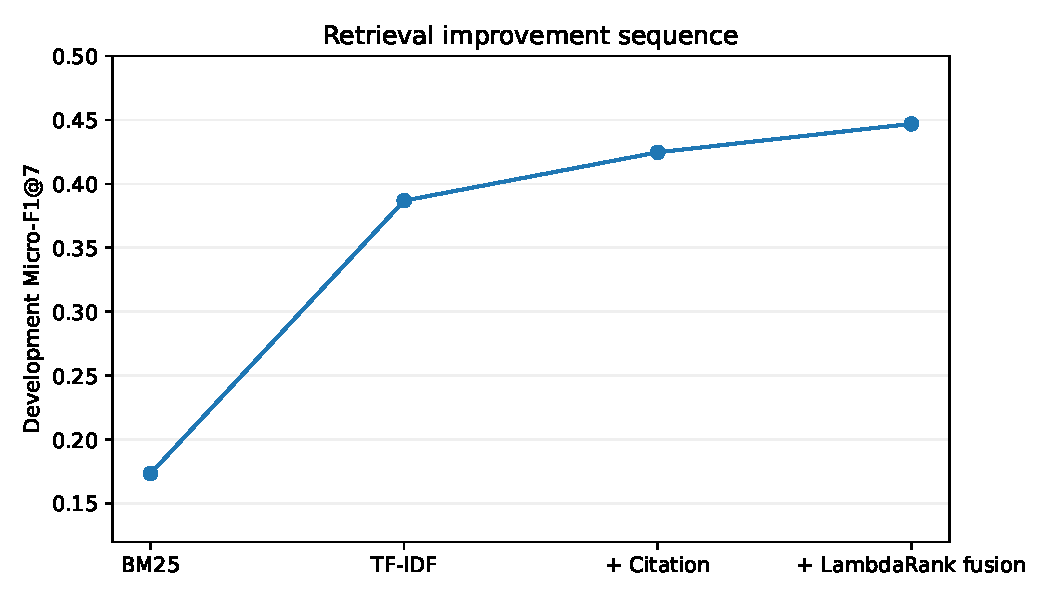
\includegraphics[width=.96\linewidth]{figures/phase7/p7_improvement.pdf}
\caption{Development improvement across E00, E07, E08 and E10. The numbers
come from the original and V2 executed-manifest records, not an unrun sweep.}
\label{fig:p7-improvement}
\end{figure}

\subsection{Experimental chronology and official Codabench evidence}
\label{subsec:p7-results}
\begin{table}[htbp]
\centering
\small
\caption{Eleven observed Phase-7 official primary scores, from the provided
Codabench screenshots (7 November 2026), paired with saved notebook development
results. E00--E06 archive-to-number assignment follows the original notebook's
submission order and remains \emph{provisional} pending byte comparison with the
renamed uploads; E07--E10 order is verified from the V2 notebook.}
\label{tab:p7-scores}
\begin{tabular}{llrr}
\toprule
Experiment & Method & Dev F1@7 & Official F1@7 \\
\midrule
E00 & BM25 & .1734 & .1949 \\
E01 & Partial fine-tuning & .2101 & .2144 \\
E02 & IA\textsuperscript{3} & .2034 & .2067 \\
E03 & LoRMA+ & .2157 & .2239 \\
E04 & Full fine-tuning & .2179 & .2268 \\
E05 & Knowledge distillation & .2101 & .2138 \\
E06 & BM25/neural ensemble & .2190 & .2209 \\
\midrule
E07 & Full-document TF--IDF & .3869 & .3839 \\
E08 & TF--IDF with citation signals & .4247 & .4265 \\
E09 & LightGBM LambdaRank & .4069 & .4253 \\
\textbf{E10} & \textbf{Citation--LambdaRank fusion} & \textbf{.4469} & \textbf{.4619} \\
\bottomrule
\end{tabular}
\end{table}

All eleven screenshots show \texttt{Finished} submissions. The final winner is
submission 1039660, uploaded as \texttt{submission11.zip} and generated by
\texttt{E10\_DEV\_SELECTED\_LEGAL\_RANKER}. Its hidden-reference
Micro-F1@7 is \textbf{0.4619}, compared with 0.4253 for the stand-alone
LightGBM run and 0.4265 for citation-enhanced TF--IDF. The displayed top
leaderboard score was 0.5162 at the time of the screenshot; no claim is
made about a lasting final rank. Official secondary metrics were not supplied
for these eleven submissions, so this report does not invent them.

\begin{figure}[htbp]
\centering
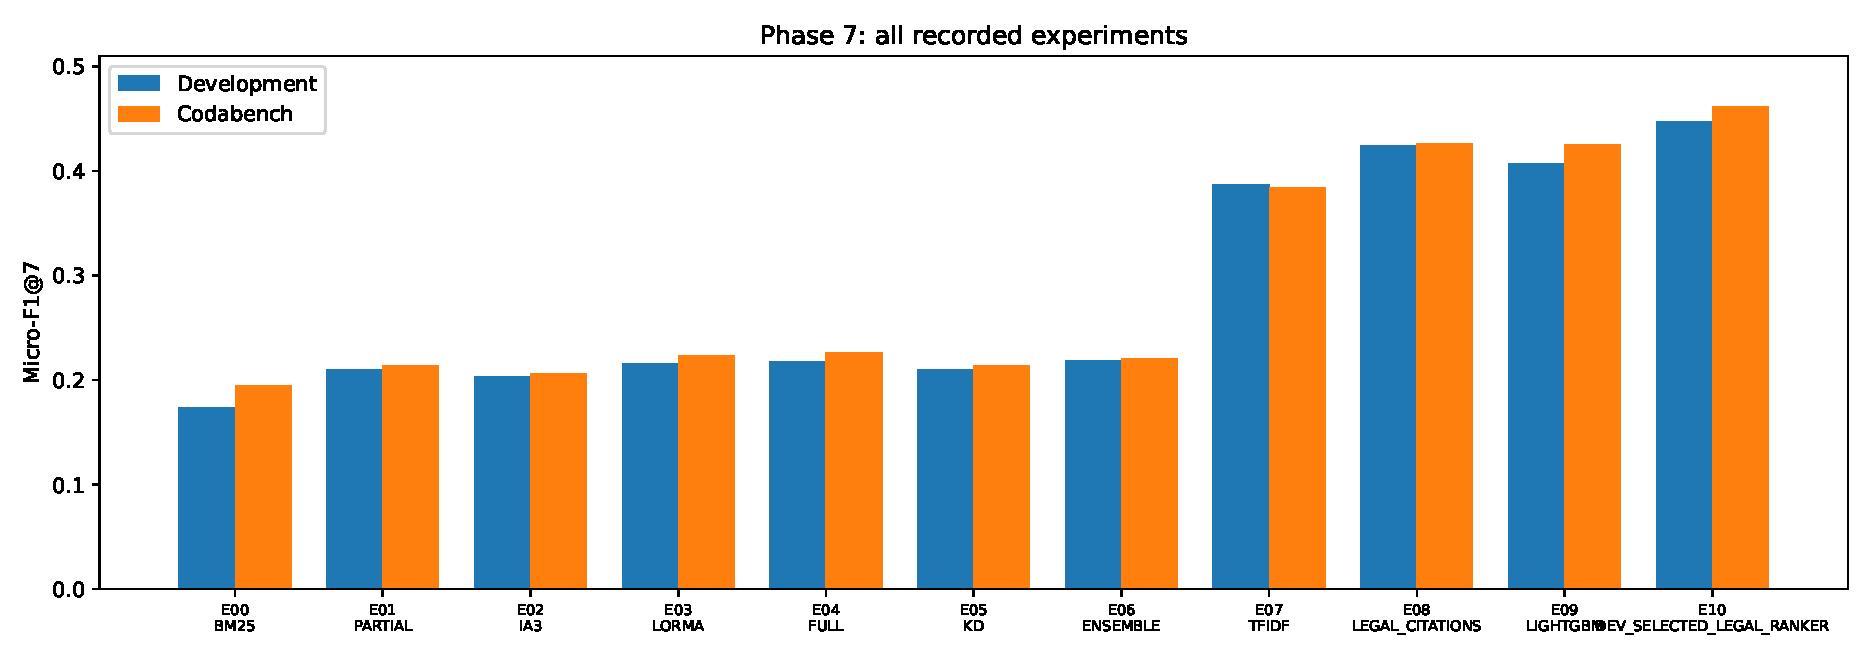
\includegraphics[width=\linewidth]{figures/phase7/p7_results.pdf}
\caption{Archived development and official Micro-F1@7 values for all eleven
historical experiment IDs. Experiment-to-upload filename mapping for the original
seven is marked provisional in the machine-readable source CSV.}
\label{fig:p7-official}
\end{figure}

\subsection{Error analysis, counterexamples and post-submission diagnostics}
\label{subsec:p7-errors}
The first-stage failure was obvious in the BM25 oracle analysis: gold cases
outside the top 256 could never be recovered. Other failures arise because
similar legal language need not imply the same controlling issue and, conversely,
a useful precedent can be lexically distant. Long documents contain boilerplate,
cited statutes and procedural narratives that may dominate whole-text
similarity. The V2 citation features provide strong precision when recognizable
metadata exist, but they fire on only a subset of relevant pairs.

Actual development examples show the gains and limits of citation matching.
Query \texttt{0001416283} has 11 gold cases; E07 recovered one in the top seven
while E08 recovered six. Query \texttt{0000092507} improved from three to
seven recovered cases out of 12 gold cases. Conversely, query
\texttt{0001673100} has four gold cases and neither E07 nor E08 recovered
any. Query \texttt{0181443842} has 92 gold cases, illustrating that even a
perfect top-seven system can retrieve only seven of its relevant precedents.
These examples are based on the actual development labels and rankings, not
synthetic illustrations.

\paragraph{Self-retrieval oversight.}
For all 118 development queries, the query's candidate document was identical
to the query source. E07 ranked the self-case in its top seven for all 118
queries; E08 did so for 113. These pairs are never gold relevant.
A separate \emph{post-submission diagnostic} masked the query ID before top-seven
ranking and recomputed the official metric. E07 improved from 0.38688 to
0.42468, while E08 improved from 0.42468 to 0.45247; this was not submitted
as a new official experiment. The E10 archived test predictions included
self-case IDs for 85 of the 237 queries. The diagnostic reveals a correctable
ranking issue, but it cannot establish a new official hidden-test score.

\begin{figure}[htbp]
\centering
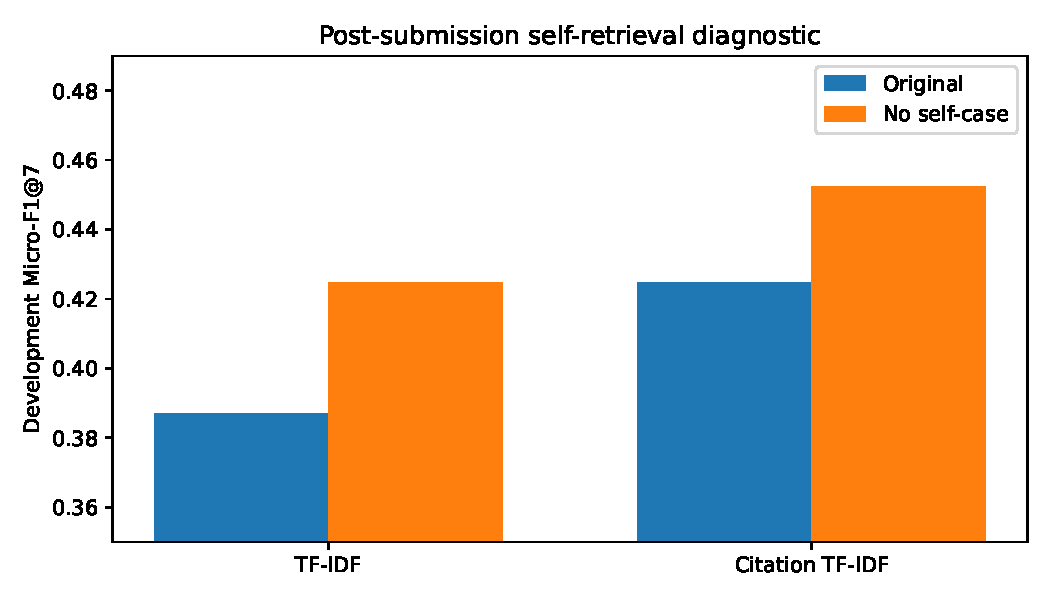
\includegraphics[width=.77\linewidth]{figures/phase7/p7_self_exclusion.pdf}
\caption{Post-submission development ablation: excluding the query case
from its own ranking. Neither masked variant has an official score.}
\label{fig:p7-self}
\end{figure}

\paragraph{Interpretation and limitations.}
The original adapter experiments establish that different degrees of Phase-1
transfer were completed, but not that full fine-tuning is inherently inferior
to sparse retrieval. The architectures used truncated inputs and were bounded
by an imperfect lexical shortlist; increasing the training budget alone may
not remove those bottlenecks. The V2 weights were selected on one 118-query
development set, so some selection noise or overfitting is possible. The
larger official improvement of E10 relative to its development score is
encouraging but not a repeated-seed or bootstrap uncertainty estimate.

Citation signals deserve particular scrutiny: \texttt{CITATOR INFO} is a
retrospective legal-publishing field. It is public text within the competition
input, not a hidden relevance label, but it may list later cases that cited
an earlier decision. A prospective legal-deployment system cannot necessarily
know future citing decisions at the moment of the query judgment. Strong
competition performance with this feature must therefore not be interpreted
as prospective prior-case retrieval performance without equivalent metadata.

\subsection{Reproducibility, software deliverables and code boundaries}
\label{subsec:p7-repro}
The research implementation provides two executable pipelines. The original
Phase-1-transfer reproduction includes E00 BM25, E01 partial fine-tuning,
E02 IA\textsuperscript{3}, E03 LoRMA+, E04 full fine-tuning, E05 distillation,
and E06 ensemble, with original hyperparameters and checkpoint resumption.
It requires the user-supplied Phase-1 tokenizer and 700M-token GQA
checkpoint; large weights are not placed in public Git.

The V2 recovery script reproduces E07--E10 with split-local TF--IDF,
citation parsing, the exact eight-feature LambdaRank input, full positive-pair
training, development selection, top-seven ranking and ZIP validation. It is
portable and accepts dataset, cache, output and model directories via
command-line arguments. The saved LightGBM pickle is an optional external
artifact for exact historical-weight replay. When absent, the script retrains
the model on the official training set. Re-execution may differ slightly with
scikit-learn/LightGBM versions or due to cached feature choices; documented
package ranges and random seed are therefore important.

The released experiment registry (\texttt{official\_results.csv}) records
all eleven official scores and source confidence, and the figure generator
recreates every Phase-7 PDF plot from checked-in aggregate data. Output JSON
is checked for exact test ID coverage, seven unique candidate IDs per query,
and ZIP root structure. Historic uploaded ZIPs and original large model
weights are not stored in the public repository. No original-weight comparison
of the complete reconstructed neural architecture was run in the present
evidence-audit environment; the historical notebook's execution and saved
checkpoint records are distinct from a fresh original-weight replay.

\subsection{Cross-phase interpretation and conclusion}
The seven tasks measure different capabilities with incomparable numeric
scales: continuation and summarization use BERTScore; named entities,
rhetorical roles, judgment prediction and statute identification use their
own classification metrics; this phase uses micro-averaged retrieval F1@7.
There is no meaningful global average of these scores. The common research
question is whether an official-data-only, self-hosted legal foundation can
be adapted efficiently to distinct legal NLP problems.

Phase 7 demonstrated both a negative and a positive result. Several
meaningful legal-LM adaptations were implemented, but in the original design
the shortlist bottleneck, underrepresented long-document evidence and sparse
positive sampling dominated the downstream ranking performance. Conversely,
full-document sparse representations and explicit legal-citation structure
proved exceptionally effective, and a carefully regularized learning-to-rank
model provided complementary judgments that improved reciprocal-rank fusion.
The official winning Micro-F1@7 was 0.4619 for E10. Future work should
compare genuine long-document dense retrievers with self-case masking, stronger
negative construction, prospective citation availability, repeated random
seeds, calibrated assessment of uncertainty, and error analysis under
realistic self-hosted deployment constraints. This closes the seven-phase
research sequence while preserving a separate, smaller final course report
as a future derivative rather than silently replacing the comprehensive
master study.
